% This file was created with tikzplotlib v0.9.12.
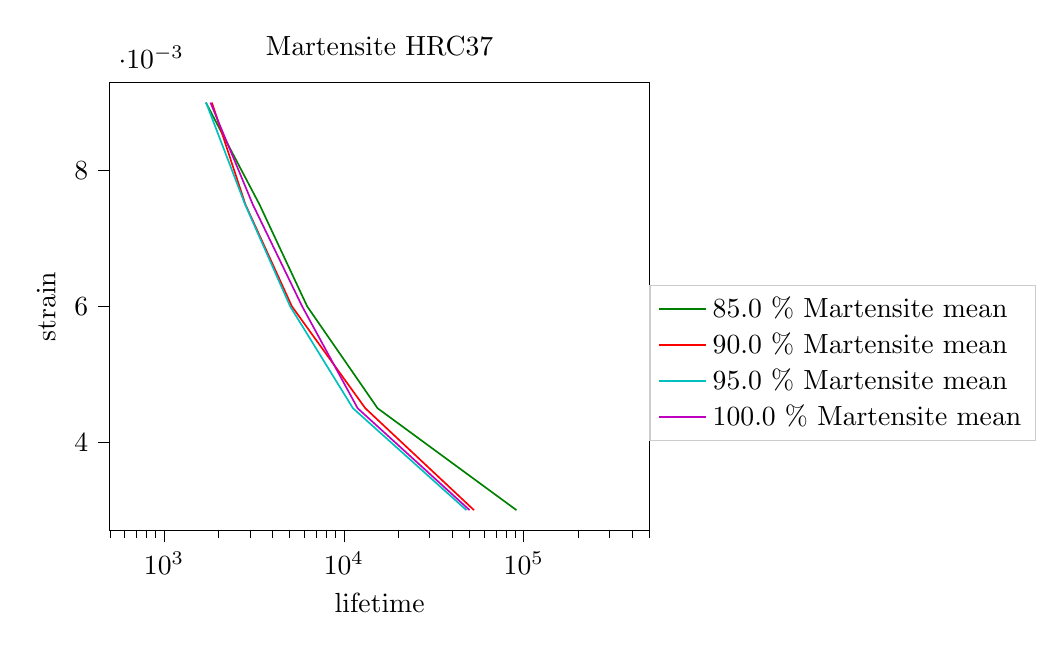
\begin{tikzpicture}

\definecolor{color0}{rgb}{0,0.75,0.75}
\definecolor{color1}{rgb}{0.75,0,0.75}

\begin{axis}[
legend cell align={left},
legend style={
  fill opacity=0.8,
  draw opacity=1,
  text opacity=1,
  at={(1,0.2)},
  anchor=south west,
  draw=white!80!black
},
log basis x={10},
tick align=outside,
tick pos=left,
title={Martensite HRC37},
x grid style={white!69.0196078431373!black},
xlabel={lifetime},
xmin=500, xmax=500000,
xmode=log,
xtick style={color=black},
y grid style={white!69.0196078431373!black},
ylabel={strain},
ymin=0.0027, ymax=0.0093,
ytick style={color=black}
]
\addplot [semithick, green!50!black]
table {%
91117.9086669353 0.003
15399.0691638736 0.0045
6253.65937638073 0.006
3396.13328458974 0.0075
1709.9778487594 0.009
};
\addlegendentry{85.0 \% Martensite mean}
\addplot [semithick, red]
table {%
52903.8502264968 0.003
13157.4225065822 0.0045
5142.21930980312 0.006
2837.01575584978 0.0075
1846.93400643699 0.009
};
\addlegendentry{90.0 \% Martensite mean}
\addplot [semithick, color0]
table {%
48017.7779215805 0.003
11237.5986258664 0.0045
5027.34367691727 0.006
2824.51515020616 0.0075
1714.42080472947 0.009
};
\addlegendentry{95.0 \% Martensite mean}
\addplot [semithick, color1]
table {%
50005.3323990349 0.003
11930.0530606028 0.0045
5865.55786010621 0.006
3117.41802638699 0.0075
1813.56617620112 0.009
};
\addlegendentry{100.0 \% Martensite mean}
\end{axis}

\end{tikzpicture}
